\chapter{Duboko učenje}
\makeatletter
\renewcommand{\ALG@name}{Algoritam}
\makeatother



Pojava i razvoj računala u drugoj polovici 20. stoljeća omogućila je automatizaciju mnogih poslova za koje su prije bili potrebni ljudi. Obrada i unos velike količine podataka, nadzor raznih proizvodnih procesa do povezivanja cijelog svijeta kroz jedinstvenu globalnu mrežu - Internet, računala su uspješno preuzela mnoge poslove za koje su prije bili nužni ljudi. No određena vrsta problema dugo je vremena izmicala pokušajima da se automatizira računalima - tzv. UI - potpuni problemi. To su problemi čija je složenost jednaka rješavanju glavnog problema umjetne inteligencije - izgradnja stroja inteligentnog poput čovjeka \citep{uilectures}. U to područje spadaju problemi poput obrade prirodnog jezika, raspoznavanja uzoraka, problemi kretanja i navigacije, te među ostalim, i područje računalnog vida. Konkretni pokušaji rješavanja ovih problema ovisili su o konkretnom problemu, te su se zasnivali na algoritamskom rješavanju problema (u području umjetne inteligencije često nazivan i simbolički pristup). Primjerice, u području računalnog vida često je bilo korištenje ručno podešenih filtera i klasifikatora za rješavanje raznih problema. No, do pravog napretka dolazi sredinom 2000-ih, pojavom dubokih neuronskih mreža, koje su uvele pravu revoluciju u područje računalnog vida.\\

\noindent U ovom poglavlju predstavit ću osnovne koncepte rada dubokih neuronskih mreža, krenuvši od opisa umjetnog neurona i jednostavne neuronske mreže, sve do složenijih dubokih modela. Također ću se osvrnuti na njihovu primjenu u području računalnog vida i problemu semantičke segmentacije, te dati primjer par najčešće korištenih arhitektura.

\section{Neuronske mreže}

Neuronsku mrežu možemo definirati kao skup međusobno povezanih procesnih jedinica (neurona) čija se funkcionalnost temelji na modelu biološkog mozga, odnosno neurona. Dakle, to je sustav koji za obradu podataka i donošenje zaključka nastoji imitirati ljudski mozak. Glavne karakteristike ovakvog pristupa, koji se često naziva i konekcionistički, su samostalno učenje na temelju predočenih podataka te mogućnost distribuirane paralelne obrade podataka. Navedene karakteristike  su u suprotnosti s algoritamskim pristupom, gdje se koraci više manje izvode slijedno, a novo znanje izvodi se pomoću predefiniranih pravila. Opis arhitekture neuronske mreže započinjemo s njenim osnovnim gradivnim elementom - neuronom. 

\subsection{Umjetni neuron}

Kako bismo bolje razumjeli model umjetnog neurona, pogledajmo prvo njegov biološki ekvivalent, kojim je i inspiriran.\\

\noindent Biološki neuroni su osnovne gradivne jedinice ljudskog mozga - prosječan ljudski mozak sadrži preko $10^{11}$ neurona, podijeljenih u preko 100 različitih vrsta. Glavni dijelovi biološkog neurona su dendriti, aksoni te tijelo (soma). 
\textbf{Dendriti} su ulazni dijelovi neurona, preko kojih neuron prima podražaje od susjednih neurona. Obrada primljenih podražaja događa se u \textbf{tijelu} neurona. U tijelu se zbrajaju sume svih podražaj primljenih preko dendrita, te se donosi odluka hoće li se neuron aktivirati ili ne. U slučaju pozitivne odluke o aktivaciji, šalje se izlazni podražaj kroz \textbf{akson} neurona.\cite{uilectures}\cite{neuroninfo}


\begin{figure}[htb]
\centering
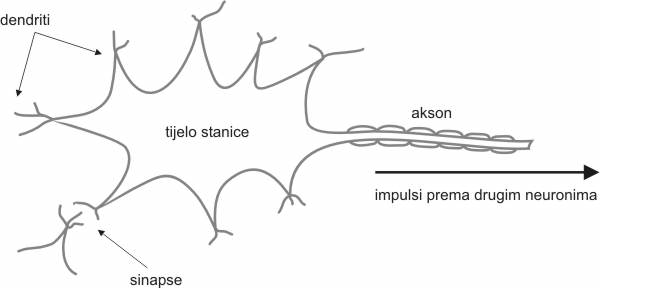
\includegraphics[width=12cm]{slike/bioloski_neuron.png}
\caption{Model biološkog neurona \citep{neuronskeMreze2008FER}}
\label{fig:fer-logo}
\end{figure}
\textbf{}
\\
Pogledamo li osnovni model umjetnog neurona, prikazan na slici 3.2, možemo primijetiti da je vrlo sličan modelu biološkog neurona. Neuron prima N numeričkih ulaza, označenih sa $\mathbf{x_{i}}$. Svakom ulazu je također pridružena i pripadajuća osjetljivost, $\mathbf{w_{i}}$, s kojom se ulaz množi prije ulaska u neuron. U neuronu se pomnoženi ulazi sumiraju, te se ukupnoj sumi dodaje pomak \engl{bias}, $\mathbf{w_{0}}$. Ovime smo definirali akumuliranu vrijednost \textit{\textbf{net}}, te ju možemo zapisati kao

\NewEnviron{myequation}{%
    \begin{equation}
    \scalebox{1.2}{$\BODY$}
    \end{equation}
    }

\begin{myequation}%
\bm{net =  (\sum\limits_{i=1}^nx_{i}   \cdot  w_{i}  )  +  w_{0}}  %
\end{myequation}


\noindent Dobivena \textit{net} vrijednost propušta se kroz \textbf{izlaznu funkciju} f \engl{activation function}, te dobivamo izlaznu vrijednost, o. \citep{uilectures}\citep{neuronskeMreze2008FER}\\

\begin{figure}[htb]
\centering
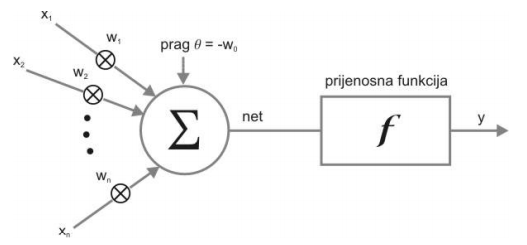
\includegraphics[width=12cm]{slike/umjetni_neuron.png}
\caption{Model umjetnog neurona \citep{neuronskeMreze2008FER}}
\label{fig:fer-logo}
\end{figure}
\textbf{}

\noindent Kako bi olakšali prikaz parametara neuronske mreže, možemo prijeći na vektorsku notaciju, gdje vektorom smatramo matricu sa točno jednim stupcem i N redaka. Onda ulaze $\mathbf{x_{i}}$ neurona možemo zapisati kao jedan vektor  $\mathbf{\overrightarrow{x} = (x_{1},x_{2}...x_{n})}$. Težine možemo prikazati vektorom $\mathbf{\overrightarrow{w} = (w_{1},w_{2}...w_{n})}$, dok pomak $\mathbf{w_{0}}$ možemo ostaviti u skalarnom obliku. Konačno, izlaz neurona o možemo zapisati kao:

\begin{myequation}%
\bm{o =  f(\overrightarrow{w}^{T} \cdot \overrightarrow{x} + b)}  %
\end{myequation}

\\
\noindent Upravo opisan model neurona se naziva TLU-perceptron \engl{Threshold logic unit}, te je prvi put predstavljen od strane McCullougha i Pittsa 1943. godine. Iako je razmjerno jednostavan, dovođenjem odgovarajućih ulaza te podešavanjem težina, pomaka i izlazne funkcije, njega već možemo koristiti za jednostavnije postupke klasifikacije i regresije. No, oni ipak imaju svoje ograničenje. To ograničenje se očituje činjenici da je \textbf{granica odluke} (skup točaka oko kojih neuron mijenja svoju odluku) TLU-perceptrona linearna, što znatno ograničava moguće primjene. Kako bismo riješili ovaj problem, prelazimo na sustave više povezanih neurona - neuronske mreže.

\subsection{Arhitektura neuronske mreže}
Neuronske mreže nisu ništa drugo osim sustavi međusobno povezanih umjetnih neurona. Svaka neuronska mreža sastoji se od više slojeva. \textbf{Sloj} je skup neurona unutar neuronske mreže koji se uvijek zajedno aktiviraju. Razlikujemo 3 vrste slojeva: ulazni sloj, skrivene slojeve te izlazni sloj.
\textbf{Ulazni sloj} služi kao ulazna točka za podatke, te uvijek postoji samo jedan.
\textbf{Izlazni sloj} je uvijek također samo jedan, te služi za izlaz iz neuronske mreže. Priroda tog izlaza ovisi o tome kako koristimo neuronsku mrežu - primjerice, koristimo li ju za klasifikaciju ulaza u N klasa, izlazni sloj može činiti N neurona, od kojih svaki kao izlaz daje vjerojatnost da ulaz pripada i-toj kasi.
\textbf{Skriveni slojevi} su glavni dio neuronske mreže, te upravo podešavanjem njihovih težina i pragova možemo neuronsku mrežu prilagoditi, odnosno naučiti nekom konkretnom problemu.
Na slici 3.3 također možemo primijetiti da svaki neuron u nekom sloju kao ulaz prima izlaze neurona iz prijašnjeg sloja. Svaka takva veza ima određenu težinu $w_{qp}$, gdje je q indeks neurona u prijašnjem sloju, a p indeks neurona u trenutnom sloju. Npr. težinu veze koja spaja neuron indeksa 1 u prijašnjem sloju te neuron indeksa 3 u trenutnom sloju mogli bismo označiti sa $w_{13}$.

\begin{figure}[htb]
\centering
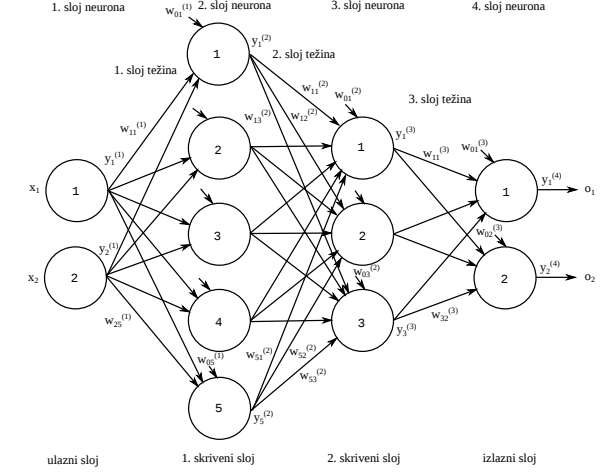
\includegraphics[width=14cm]{slike/neuronska_mreza_full.png}
\caption{Arhitektura neuronske mreže 2 x 5 x 3 x 2 \citep{umjetneNNJava}}
\label{fig:fer-logo}
\end{figure}
\textbf{}

\noindent Izlaz određenog neurona ovisi o vrijednosti izlaza neurona iz prošlog sloja, težine između trenutnog i prošlog neurona te vrijednosti praga u neuronu. Ovakve mreže, gdje izlaz neurona trenutnog sloja ovisi isključivo o izlazima neurona prethodnog sloja nazivamo \textbf{slojevitima}. Uz njih, postoje i \textbf{neslojevite} neuronske mreže, gdje izlaz neurona u nekom sloju može ovisiti o nekom neuronu više slojeva prije, ili čak o neuronu u nekom od sljedećih slojeva. Međutim, ovakve neuronske mreže nas trenutno ne zanimaju, te se u nastavku rada bavimo samo sa unaprijednim slojevitim neuronskim mrežama. \\

\noindent Sada nas još zanima kako doći do izlaza određenog sloja neuronske mreže. Kako bi olakšali zapis parametara neuronske mreže, kao i kod umjetnog neurona uvodimo vektorski zapis.
Matricu težina između i-tog i (i-1) sloja neuronske mreže možemo zapisati kao $\mathbf{W_{i}}$. Vrijednost u i-tom retku te j-tom stupcu matrice označava vrijednost težine između i-tog neurona trenutnog sloja te j-tog neurona prethodnog sloja. Ukoliko još sa $\mathbf{b_{i}}$ označimo pragove i-tog sloja neurona, izlaz i-tog sloja neuronske mreže, $h_{i}$, možemo zapisati kao:

\begin{myequation}%
\bm{\overrightarrow{h_{i}} =  f(W_{i} \cdot \overrightarrow{h_{i-1}} + b_{i})}  %
\end{myequation}

\noindent gdje je f izlazna funkcija \citep{uilectures}. Drugim riječima, izlaz svakog sloja neuronske mreže jednak je skalarnom produktu matrice težina sloja i izlaza prethodnog sloja, na koji još dodamo vektor pragova trenutnog sloja. Nad dobivenim vektorom primijenimo izlaznu funkciju, te smo dobili izlazni vektor sloja, u kojem i-ti stupac odgovara izlazu i-tog neurona u sloju. Ukoliko se radi o prvom skrivenom sloju, vektor $h_{i-1}$ je ustvari samo ulazni vektor. Vidimo da, kako bi u potpunosti definirali našu mrežu, potreban nam je vektor težina, vektor pragova i prijenosna funkcija za svaki od slojeva. Modifikacijom nekog ili svih parametara možemo promijeniti izlaz naše mreže. Upravo modifikacija navedenih parametara je jedan od ključnih dijelova u procesu učenja odnosno treniranja mreže, detaljnije obrađenog u sljedećem potpoglavlju.\\

\noindent Zadnja stvar koju je bitno napomenuti je odabir odgovarajuće prijenosne funkcije. Ako želimo da naša mreža bude ekspresivnija od običnog neurona, odnosno ako želimo modelirati i nelinearne odnose, nužno je koristiti nelinearnu prijenosnu funkciju. To je rezultat činjenice da je linearna kombinacija linearnih kombinacija također linearna kombinacija. Odnosno, ako primijenimo linearnu prijenosnu funkciju na izlaz sloja neuronske mreže, koji je i sam linearna kombinacija težina i ulaza, kao rezultat možemo dobiti samo novu linearnu kombinaciju. Najčešće korištene prijenosne funkcije uključuju sigmoidu, tangens hiperbolni, softmax i reLU, od kojih je posljednja posebice korisna prilikom treniranja dubokih modela.\citep{uilectures} 



\noindent 


\subsection{Učenje neuronskih mreža}
Učenje neuronskih mreža svodi se na mijenjanje jakosti veza između neurona - dakle na podešavanje vrijednosti pragova i težina neurona unutar mreže. Te parametre prilagođavamo kroz iterativan postupak predočavanja ulaznih primjera, najčešće u kombinaciji s očekivanim izlazom - treniranje. Stoga možemo zaključiti da je znanje o izlazu kao funkciji izlaza unutar neuronske mreže pohranjeno implicitno, kroz pragove i težine između neurona. To rezultira time da neuronske mreže najčešće funkcioniraju po principu crne kutije - za dani ulaz, vraćaju odgovarajući izlaz, međutim način na koji je neuronska mreža došla do tog izlaza je teško opisati. Takav način pohrane znanja o mapiranju ulaza na izlaze u suprotnosti je algoritamskim pristupom, gdje točno možemo opisati svaki korak pomoću kojeg smo došli do izlaza.\citep{neuronskeMreze2008FER} \\

\noindent Prije nego detaljnije opišemo postupak učenja, napomenimo da najčešće razlikujemo 3 vrste učenja. Prva, najčešće korištena metoda u svijetu dubokog učenja, je \textbf{nadzirano} \engl{supervised} učenje. Glavna karakterisika ove metode je da modelu, u ovom slučaju neuronskoj mreži, dajemo parove (ulaz, izlaz). Sustav zatim pokušava konstruirati funkciju koja će što točnije moći preslikati dani ulaz na očekivani izlaz. Druga metoda je \textbf{nenadzirano} \engl{unsupervised} učenje. U ovoj metodi modelu dajemo samo određen broj ulaza, bez pripadajućih izlaza, i modelu prepuštamo da pronađe pravilnost u podacima. Ova metoda se može primijeniti u kombinaciji sa nadziranim učenjem. Baš tu kombinaciju ćemo pobliže istražiti u nastavku ovog rada. Treća i ujedino posljednja vrsta učenja je \textbf{podržano} \engl{reinforcement} učenje. Glavni cilj ovog načina učenja je doći do niza koraka, odnosno strategije, koja rješava neki problem. 
U nastavku ćemo pogledati primjer nadziranog učenja neuronskih mreža uz pomoć jednog od najčešće korištenih algoritama - \textbf{algoritma propagacije pogreške unazad} \engl{error backpropagation}.

Kako bi objasnili algoritam, potrebno je uvesti još par pojmova. Prvi je pojam \textbf{funkcije pogreške} \engl{loss function}, često nazivane i funkcija gubitka. Već smo spomenuli da se, u svojoj osnovi, treniranje neuronskih mreža svodi na predočavanje ulaznih primjera te usporedbom dobivenog izlaza s očekivanim izlazom. Na temelju razlike između očekivanog i dobivenog izlaza modificiraju se parametri mreže. Međutim, ostaje pitanje kako točno kvantificirati razliku između ta dva izlaza? Za to nam služe funkcije gubitka. To su funkcije koje na osnovu očekivanog i dobivenog izlaza računaju jedinstvenu numeričku vrijednost pogreške. Očito, model je bolji što je vrijednost funkcije pogreške manja, stoga se učenje modela u praktičnoj primjeni zasniva na minimizaciji funkcije pogreške. U teoriji, model u kojem je svaki dobiveni izlaz jednak svakom očekivanom izlazu bi imao vrijednost funkcije pogreške jednaku 0.

Jedna od češće korištenih funkcija gubitka je (polovična) suma srednjih kvadratnih odstupanja \engl{Mean Squared Error, MSE}, koju definiramo kao:

\begin{myequation}%
\bm{MSE = \frac{1}{2N} \sum\limits_{s=1}^N \sum\limits_{i=1}^{ N_{0} }  {( t_{s,i} -  o_{s,i})} }^{2}   %
\end{myequation}

\noindent pri čemu $s$ označava redni broj para (očekivani izlaz, dobiveni izlaz), $N$ broj takvih parova, $N_{0}$ dimenziju izlaza, $t$ očekivani izlaz i $o$ dobiveni izlaz. Kvadrat u izrazu služi kako bi osigurali da će dobivena vrijednost uvije biti pozitivna, neovisno o tome je li očekivani izlaz manji ili veći od dobivenog.\\

\noindent Prisjetimo se na trenutak matematičke analize i pojma gradijenta funkcije - vektora nastalog parcijalnom derivacijom funkcije po svim njenim varijablama. On ima korisno svojstvo - pokazuje nam smjer najbržeg rasta funkcije. Jednom kada smo izračunali gradijent funkcije, možemo ga iskoristiti za minimizaciju funkcije korištenjem \textbf{tehnike gradijentnog spusta} \engl{gradient descent}. Tehnika se sastoji od malih modifikacija svake varijable funkcije u smjeru suprotnom od onog u kojem pokazuje gradijent. Ova tehnika nam garantira eventualni dolazak u neki od lokalnih minimuma funkcije. \citep{deeplearningbook}
Ova ideja se sad lako može primijeniti na funkciju gubitka neuronske mreže - funkcija gubitka je funkcija čiju vrijednost želimo minimizirati, a parametri koje prilagođavamo su upravo parametri neuronske mreže - težine i pragovi. To je upravo osnovna ideja algoritma propagacije pogreške unazad, čiju točnu definiciju dajem u nastavku. Algoritam je preuzet iz \citep{umjetneNNJava}, te pretpostavlja da je korištena sigmoidalna prijenosna funkcija:




\begin{algorithm}
  \caption{Algoritam propagacije pogreške unazad}


  
  \begin{algorithmic}
    \Statex
      1. Sve težine neuronske mreže postavi na slučajne vrijednosti
      2. \While{ uvjet zaustavljanja nije zadovoljen}:
      \Repeat
      \For{svaki uzorak $s$ iz skupa za učenje}
            \State 1. Postavi podatak $\bm{x}$ na ulaz mreže
            \State 2. Izračunaj izlaze neurona svih slojeva, od prvog prema posljednjem
            \State \hspace{1em}(izlaz posljednjeg sloja označimo sa $(o_{S,1}, ... o_{S,N_{0}})$
            \State 3. Odredi pogrešku svakog od neurona izlaznog sloja
            \State \hspace{1em} S $\delta ^{k}_{i}$ označimo pogrešku i-tog sloja te ju računamo prema izrazu:
            \State \hspace{1em} $\bm{\delta ^{K}_{i}  = o_{s,i} \cdot (1-o_{s,i}) \cdot (t_{s,i}-o_{s,i})}$, gdje je
            \State \hspace{1em} $(t_{s,i}-o_{s,i})$ - odstupanje između dobivenog i očekivanog izlaza, a
            \State \hspace{1em} $o_{s,i} \cdot (1-o_{s,i})$ - derivacija prijenosne funkcije neurona (sigmoida)
            
            \State 4. Vraćaj se sloj po sloj prema početku mreže i za svaki neuron i
            \State \hspace{1em} u sloju k računaj pogrešku prema izrazu:
            \State \hspace{1em} $\bm{\delta ^{k}_{i}  = y^{k}_{i} \cdot (1-y^{k}_{i}) \cdot   \sum\limits_{d \epsilon Downstream}^{} w_{i,d} \cdot \delta ^{k+1}_{d}}$
            \State 5. Napravi korekciju svih težina. Težinu $w^{k}_{i,j}$ korigiraj prema izrazu
            \State \hspace{1em} $\bm{w^{k}_{i,j}  \leftarrow w^{k}_{i,j} +  \eta \cdot y^{k}_{i} \cdot  \delta^{k+1}_{d}}$
            \State \hspace{1em} gdje $\eta$ predstavlja stopu učenja modela
        \EndFor
      \EndWhile
  \end{algorithmic}
\end{algorithm}

\subsection{Regularizacija i optimizacija}

Sada kada znamo osnove arhitekture i treniranja umjetnih neuronskih mreža, osvrnimo se na još dva pojma važna za izgradnju kvalitetnog modela - regularizacija i optimizacija.\\

\noindent \textbf{Regularizacija} je tehnika korištena prilikom treniranja modela koja kao cilj ima smanjiti pogrešku generalizacije modela, odnosno smanjiti prenaučenost \engl{overfitting}, ali pritom ne utjecati na pogrešku prilikom treniranja.\citep{deeplearningbook}. Regularizacija postaje sve važnija kako idemo prema dubokim, složenijim modelima, jer povećanjem složenosti modela njegova tendencija prenaučenosti raste. Najčešće korištene tehnike su augmentacija podataka te L1 i L2 regularizacija. 

\textbf{Augmentacija podataka} \engl{data augmentation} je jednostavan, ali vrlo moćan oblik regularizacije. Njegova osnovna ideja je kroz razne vrste manipulacija na umjetan način povećati broj uzoraka korištenih za treniranje. Povećanje broja uzoraka kao direktnu posljedicu ima bolju generalizaciju modela. Konkretan način augmentacije podataka ovisi o podacima koje koristimo, no primjerice ako koristimo 2D slike kao ulaz, augmentacija može uključivati razne manipulacije poput invertiranja slika, slučajnog obrezivanja dijelova slika ili dodavanja šuma.

Osnovna ideja \textbf{L1 i L2 regularizacija} je modifikacija funkcije gubitka tako da joj se doda određena dodatna vrijednost, koja ima cilj penalizirati prenaučeni model. Bez ulaženja u detalje, bez te dodatne vrijednosti model bi težio savršenoj prilagodbi podacima za treniranje, te bi loše generalizirao. Dodavanjem tog penala model "odmičemo" od pozicije u kojoj je savršeno prilagođen podacima za treniranje prema poziciji u kojoj će bolje generalizirati. Glavna razlika između L1 i L2 regularizacije je u načinu izračuna vrijednosti spomenutog penala. Konkretno, izraz za L1 je:

\begin{myequation}%
\bm{\sum\limits_{j=1}^N |w_{j}| }   %
\end{myequation}

Vidimo da se penal izračunava kao suma absolutnih vrijednosti težina mreže.  S druge strane L2 regularizaciju definiramo kao:

\begin{myequation}%
\bm{\sum\limits_{j=1}^N (w_{j})^2 }   %
\end{myequation}

Penal se izračunava kao suma kvadrata težina mreže. Konačni izraz za funkciju pogreške E prilikom korištenja L1 ili L2 regularizacije je onda:

\begin{myequation}%
\bm{E_{reg} = E_{orig} + \lambda(L) }   %
\end{myequation}

gdje je $\lambda$ parametar pomoću kojeg možemo modificirati jakost utjecaja regularizacije, a L korištena L1 ili L2 regularizacija.\citep{optimizationAndRegularization}

\noindent \textbf{Optimizacija} u kontekstu učenja neuronskih mreža najčešće podrazumijeva optimizaciju gradijentnog spusta, ključnog dijela učenja.

Jedan pristup optimizaciji gradijentnog spusta je kroz varijaciju količine podataka korištene u izračunu gradijenta funkcije pogreške. Osnovna varijanta gradijentnog spusta računa gradijent te provodi optimizaciju parametara na osnovu cijelog skupa podataka za treniranje. Ovo kao posljedicu može imati unošenje redundancije, jer će se gradijenti za slične ulazne primjere računati nekoliko puta prije ažuriranja parametara. \textbf{Stohastički gradijentni spust} provodi izračun gradijenta nakon svakog ulaznog primjera. To kao posljedicu ima ubrzanje konvergencije prema lokalnom minimumu, no također rezultira većom fluktuacijom vrijednosti funkcije pogreške.
Kombinacija ova dva pristupa je \textbf{gradijentni spust nad podskupu podataka} \engl{mini-batch gradient descent}. Ovaj pristup provodi izračun gradijenta i ažuriranje parametara modela nakon svakog podskupa svih podataka za učenje. Kako veličinu tog podskupa možemo lako mijenjati, ovo nam omogućava laku kontrolu gradijentnog spusta ovisno o konkretnom problemu koji rješavamo. \citep{gradientOptimizationAlgorithms}

Druge metode optimizaciji su znatno složenije, te uključuju metode poput Momentuma, AdaGrada, AdaDelte, i drugih. Jedan od najčešće korištenih je \textbf{Adam} \engl{Adaptive Moment Estimation}, koji ćemo ovdje ukratko opisati. Kao što smo vidjeli u Algoritmu 1, algoritam propagacije pogreške unazad, zasnivan na tehnici gradijentnog spusta, prilikom korekcije težina koristi parametar $\eta$ - stopa učenja. On određuje u kojoj mjeri će se parametri modela promijeniti - što je $\eta$ veći, to je promjena veća te model brže konvergira prema minimumu. Klasična tehnika gradijentnog spusta, pa čak i stohastičkog gradijentnog spusta koristi samo jedan $\eta$ za sve težine u modelu, te je on konstantan tijekom cijelog učenja modela. Adam, te algoritmi na kojima se on zasniva (AdaGrad i RMSProp) računa zaseban $\eta$ za svaki parametar mreže. Za računanje vrijednosti $\eta$, Adam koristi prosjek momenta prvog reda gradijenta (prosjek), ali i prosjek moment drugog reda (varijanca). \citep{AdamMachineLearningMastery} U praksi, Adam se pokazao najboljim, te se preporučuje njegova primjena. \citep{gradientOptimizationAlgorithms}

\section{Duboko učenje}
Duboko učenje, usprkos svom pomalo misterioznom i intrigantnom nazivu, zapravo nije ništa drugo već primjena dubokih neuronskih mreža na razne vrste problema. Pod pojmom \textbf{duboke neuronske mreže} najčešće podrazumijevamo bilo koju unaprijednu neuronsku s većim brojem skrivenih slojeva. Iako ne postoji točna definicija koliko slojeva neuronska mreža mora imati kako bismo ju smatrali dubokom, često se uzima uvjet od 3 ili više (skrivenih) slojeva. \citep{IBMDeepLearning}

Iako ideja dodavanja većeg broja slojeva u neuronske mreže nije ni u kojem smislu nova (prve "duboke" neuronske mreže pojavljuju se već 1990-ih godina), glavna prepreka koja je dugo kočila razvoj ovog područja je bio nedostatak adekvatnog hardvera. Razvojem adekvatnog hardvera u drugoj polovici 2000-ih te u 2010-im godinama omogućio je adekvatne resurse potrebne za treniranje i rad dubokih neuronskih mreža. Odjednom je bilo moguće trenirati dublje modele nego prije, te za treniranje koristiti skupove podataka nekoliko redova veličine iznad dotadašnjih, što je rezultiralo puno boljim rezultatima. Sve ovo je kao posljedicu imalo pravu renesansu u području dubokih neuronskih mreža, koje je ubrzo postalo najpopularnije i najbrže rastuće područje strojnog učenja. \citep{deeplearningbook}

Duboko učenje danas ostvaruje odlične rezultate u brojnim područjima primjene. Primjerice, desetak godina prije navedenih napredaka u dubokom učenju, područje raspoznavanja govora je stagniralo. Primjena metoda dubokog učenja rezultirala je u znatnom smanjenju pogrešaka modela, u nekim slučajevima i preko 50\%. Duboke mreže također postižu sjajne rezultate u području računalnog vida, primjerice u poljima semantičke segmentacije ili klasifikacije.

U nastavku ćemo se fokusirati na primjenu dubokog učenja na računalni vid, specifičnije na semantičku segmentaciju. Razmotrit ćemo jednu posebnu vrstu dubokih neuronskih mreža posebno prikladnih za ovaj problem - duboke konvolucijske mreže.


\subsection{Konvolucijske neuronske mreže}
Naša motivacija za uvođenje konvolucijskih neuronskih mreži je rješavanje problema iz domene računalnog vida. Glavni izvor podataka u tom području je naravno 2D slika. Ako želimo primijeniti duboko učenje na problem iz domene računalnog vida, moramo pronaći način kako 2D slike predati kao ulaz u model. Jedan naivan pristup bi mogao biti pretvoriti cijelu sliku u niz piksela, te svaki piksel dovesti kao jedan ulaz u mrežu. Zasigurno, mreža s takvim ulazima na raspolaganju ima sve podatke koji joj ikad mogu trebati! No uzmemo li u obzir da prosječna slika dimenzija 1980x1080 ima preko 2 milijuna piksela, vidimo gdje nastaje problem. Ovakav pristup bi podrazumijevao da samo ulazni sloj naše mreže ima 2 milijuna neurona - da ne spominjemo ostale slojeve. Treniranje i rad s ovakvom mrežom  u praksi bi bili nemogući. Također, ovakav pristup praktički ignorira povezanost između susjednih piksela - npr. na slici koja prikazuje nebo, puno je veća vjerojatnost da u blizini jednog piksela plave boje pronađemo još piksela plave boje, nego primjerice piksel crvene boje. Očito je da moramo promijeniti naš pristup ovom problemu.\\

\noindent \textbf{Konvolucijske neuronske mreže} \engl{convolutional neural networks, CNNs} su specijalizirana vrsta umjetnih neuronskih mreža koje karakterizira upotreba konvolucije (specijalne vrste funkcije) umjesto matričnog množenja u barem jednom od svojih slojeva. Ova vrsta mreža je posebno dobra u obradi podataka sa mrežastom topologijom - uz što među ostalim spadaju i 2D slike. \citep{deeplearningbook} Konvolucijske neuronske mreže se sastoje od 3 glavna sloja - konvolucijski, sloj sažimanja i potpuno povezani sloj. Rad konvolucijskih mreža objasnit ćemo na primjeru rada svakog od navedenih slojeva.\\

\noindent \textbf{Konvolucijski sloj} \engl{convolutional layer} je sloj čija je glavna zadaća ekstrakcija značajki iz originalne slike (ili pak iz izlaza prethodnog konvolucijskog sloja). Te značajke su primjerice rubovi, određene boje ili linije unutar slike. Ključni pojam u ovom sloju je \textbf{jezgra} \engl{kernel}. U svojoj osnovi, jezgra je filter koji prolazi kroz originalnu sliku, dio po dio, te na svakom od tih dijelova provodi operaciju konvolucije. \textbf{Konvolucija} je operacija nad dvjema funkcijama, f i g, čiji je rezultat treća funkcija koja opisuje kako funkcija f utječe na oblik funkcije g. \citep{convolutionOperationsCNN}  Konkretno u našem primjeru, funkcija f bi bila jezgra (odnosno filter), a funkcija g originalna slika. Konvolucija se provodi jednostavnim matričnim množenjem i zbrajanjem dijela ulazne matrice (slike) koji se trenutno promatra i jezgre. Veličina ulazne matrice jednaka je veličini jezgre, dok je veličina pomaka po ulaznoj matrici određen parametrom koji nazivamo \textbf{korak} \engl{stride} - što je korak veći, izlaz konvolucijskog sloja će biti manjih dimenzija, i obratno. Rezultat konvolucije, odnosno primjene filtera na neki dio slike nam može dati informaciju je li element za koji je taj filter zadužen prisutan na tom dijelu slike ili ne. Primjerice ako se radi o filteru zaduženom za ekstrakciju rubova, mogao bi pridijeliti veće vrijednosti dijelovima slike na kojima se nalaze rubovi, a manje onima na kojima ne, tražeći mjesta gdje dolazi do nagle promjene svjetline ili intenziteta boja. Rezultat provođenja ove operacije, odnosno izlaz ovog sloja je nova matrica, manjih dimenzija od ulazne, koju zovemo  \textbf{mapa značajki}. Važno je napomenuti da ako se ulazna slika sastoji od više kanala (primjerice RGB format), jezgra se mora sastojati od istog broja kanala, odnosno u primjeru za RGB format od 3 zasebna filtera, po jedan za svaki od kanala. U tom slučaju izlazna mapa značajki također ima 3 kanala. Taj parametar se naziva \textbf{dubina} jezgre. Učenjem konvolucijske mreže, vrijednosti jezgre se modificiraju kako bi preslikavanje ulaza na izlaznu mapu značajki bilo točnije. Postupak konvolucije je prikazan na slici 3.4, gdje se također može primijetiti da veličina izlazne mape značajki ovisi o dimenziji ulaza te o dimenziji filtera.\\

\begin{figure}[htb]
\centering
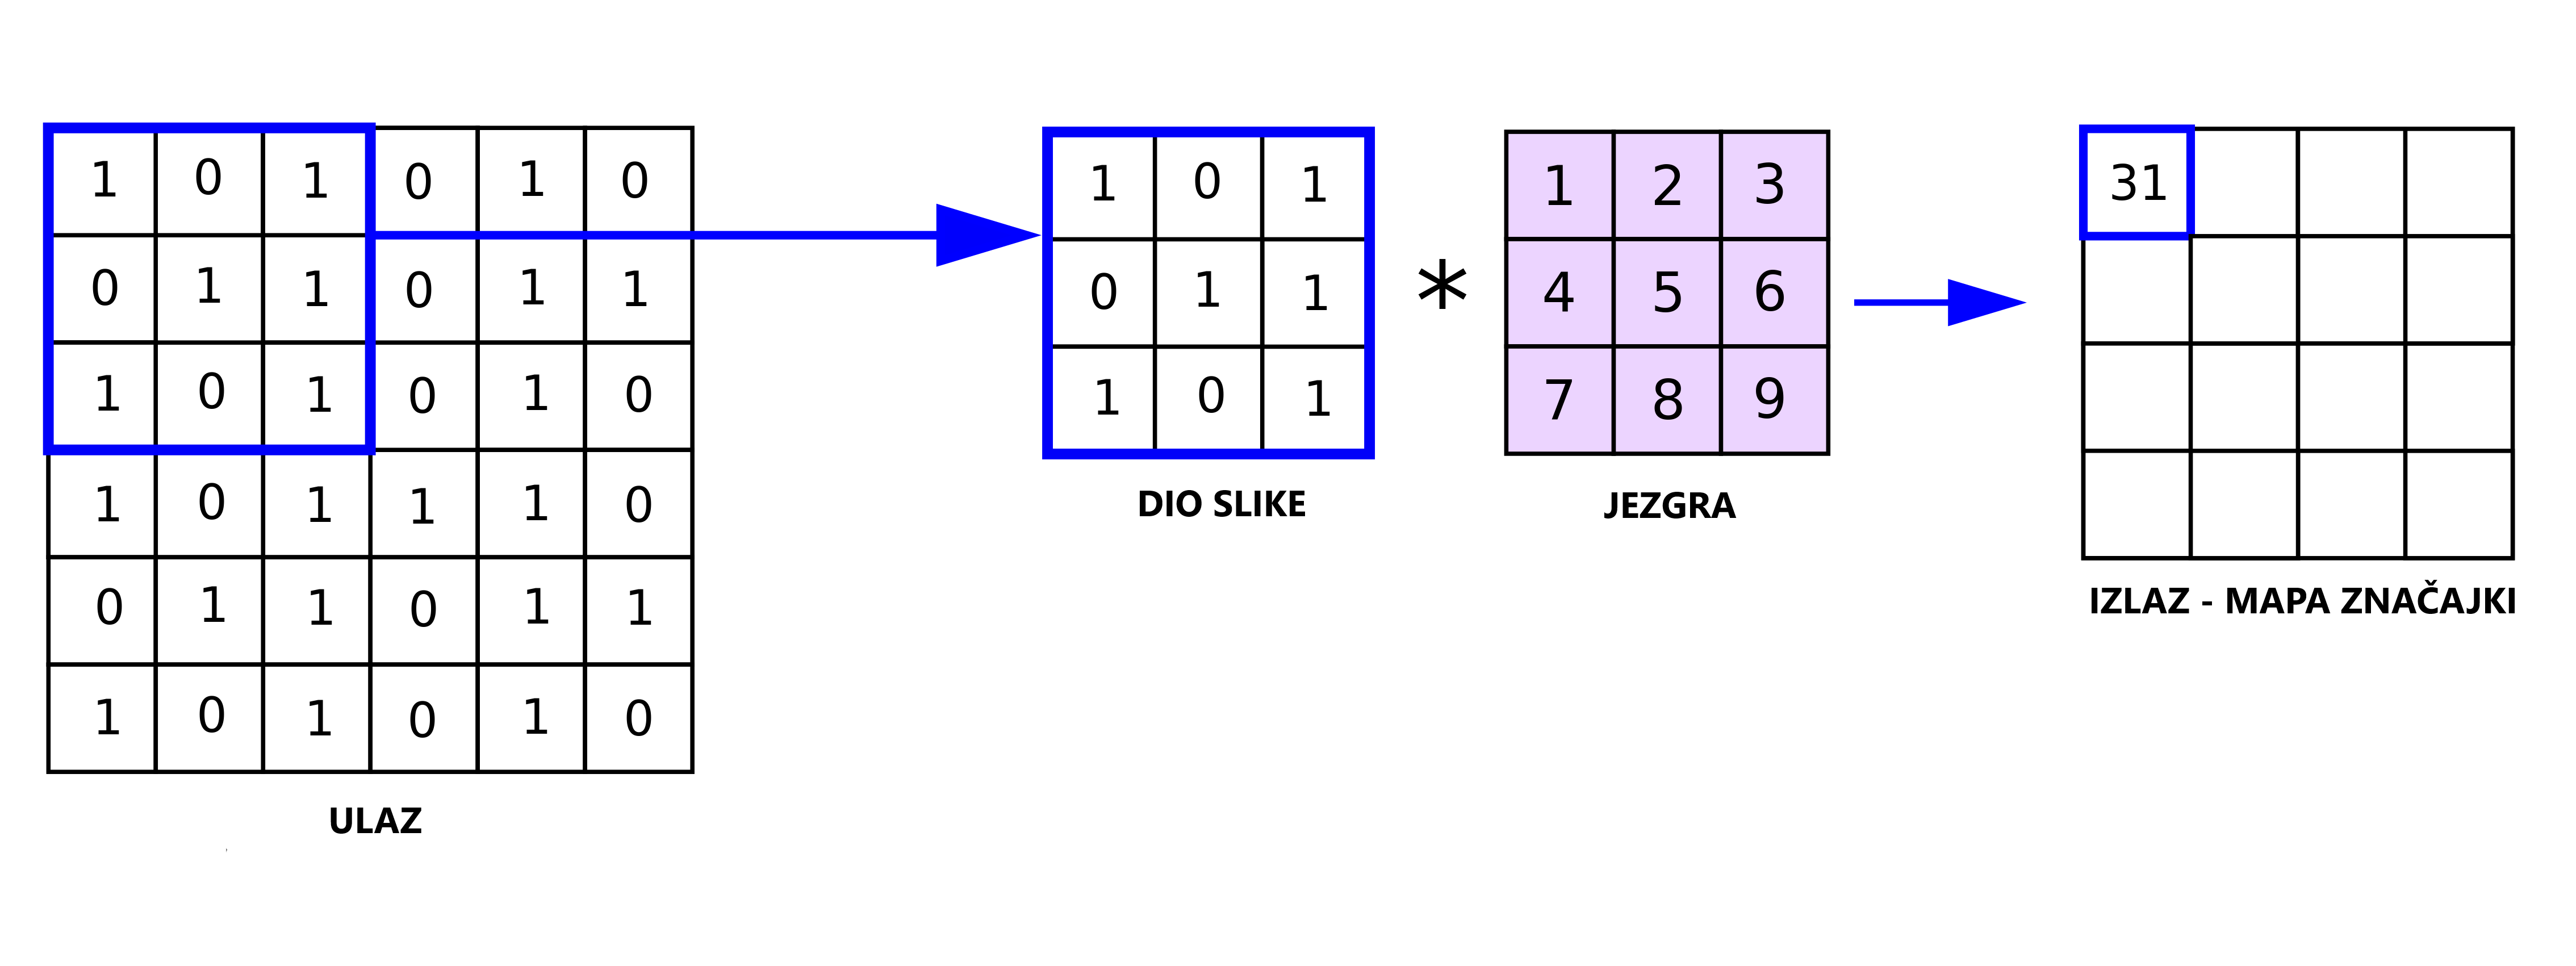
\includegraphics[width=15cm]{slike/kernelCNN.png}
\caption{Operacija konvolucije u CNN-u \citep{CNNAnnReynolds}}
\label{fig:fer-logo}
\end{figure}
\textbf{}


\noindent Nakon svakog konvolucijskog sloja, nad dobivenom mapom značajki primjenjuje se neka aktivacijska funkcija, koja je nužno nelinearna. Ako se sjetimo poglavlja 3.1.3, znamo da je nelinearnost aktivacijske funkcije bitna kako bi mreža bila u stanju modelirati složenije pojave. Najčešće korištena aktivacijska funkcija u konvolucijskim mrežama je \textbf{ReLU} \engl{Rectified Linear Units}. U svojoj osnovi, ReLU je vrlo jednostavna funkcija:

$$ReLU(x) =\begin{cases}0 & x  \leq  0\\x & x > 0\end{cases} $$

\noindent Glavne prednosti ReLU nad ostalim nelinearnim aktivacijskim funkcijama, poput sigmoide ili tangensa hiperbolnog su 

\begin{enumerate}
  \item Vrlo lagan izračun u odnosu na alternative - samo treba odrediti je li x veći ili manji od 0
  \item Derivacija ReLU je uvijek 0 ili 1. Ovo je izuzetno korisno u rješavanju problema tzv. nestajućeg gradijenta \engl{vanishing gradient}, koji je karakterističan za neke funkcije poput sigmoide. Problem se javlja zbog činjenice da derivacije sigmoidalnih funkcija teže 0 kada x -> $\infty$. ReLU, čija je derivacija uvijek 0 ili 1 nema takav problem, čime se omogućuje algoritmu propagacije pogreške da nastavi čak i za velike ulazne vrijednosti.  \citep{baeldungReLU}
\end{enumerate}

\noindent \textbf{Sloj sažimanja} \engl{pooling layer} ima kao cilj smanjiti dimenziju mape značajki, te time smanjiti broj parametara i resursne zahtjeve modela. Također ima za ulogu učiniti model manje osjetljivim na manje promjene u ulazima, time poboljšavajući generalizaciju modela. Veličinu dijela mape značajki nad kojim se provodi sažimanje određuje \textbf{dimenzija sažimanja}, dok veličinu pomaka, kao i kod konvolucijskog sloja, određuje \textbf{korak}. Naravno, veličina koraka u ovom sloju nije ni na koji način povezana s veličinom koraka u konvolucijskom sloju. Sam postupak sažimanja je vrlo sličan postupku u konvolucijskom sloju - idemo po dijelovima mape značajki, te za svaki dio računamo sažetak koristeći funkciju sažimanja. Sažetak zatim mapiramo na izlaz ovog sloja.

Razlikujemo dvije vrste sažimanja - \textbf{sažimanje po maksimalnoj vrijednosti} \engl{max pooling} te \textbf{sažimanje po prosječnoj vrijednost} \engl{average pooling}. Sažimanje po maksimalnoj vrijednosti za svaki dio ulaza (mape značajki) vraća njegovu maksimalnu vrijednost kao izlaz. Sažimanje po prosječnoj vrijednosti za svaki dio ulaza vraća njegovu prosječnu vrijednost. Između ova dva pristupa, preporučuje se korištenje sažimanja po maksimalnoj vrijednosti, jer uz smanjenje dimenzionalnosti, pridonosi i uklanjanju šuma iz ulaza. \cite{towardsDSCNN} \\

\begin{figure}[htb]
\centering
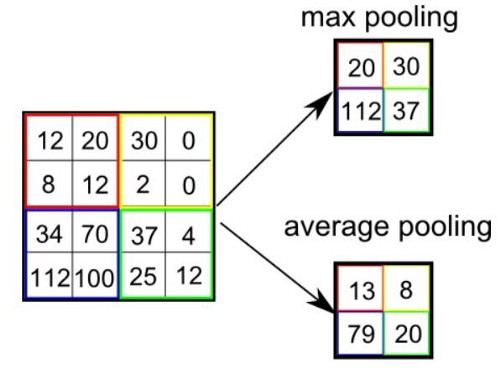
\includegraphics[height=6cm]{slike/poolingLayer.png}
\caption{Sloj sažimanja \citep{towardsDSCNN}}
\label{fig:fer-logo}
\end{figure}
\textbf{}

\noindent U nekim primjenama, primjerice klasifikacija slika, dodaje se i treći sloj, tzv. \textbf{potpuno povezani sloj} \engl{fully connected layer}. Ovaj sloj se nalazi pri kraju mreže, te na njega dolaze izlazi prethodna dva sloja, najčešće pretvoreni u jednodimenzionalni vektor. Ovaj dio konvolucijske mreže se zatim ponaša kao obična neuronska mreža.

\noindent Sve slojeve konvolucijske neuronske mreže možemo vidjeti na slici 3.6\\



\begin{figure}[htb]
\hspace{-2cm}
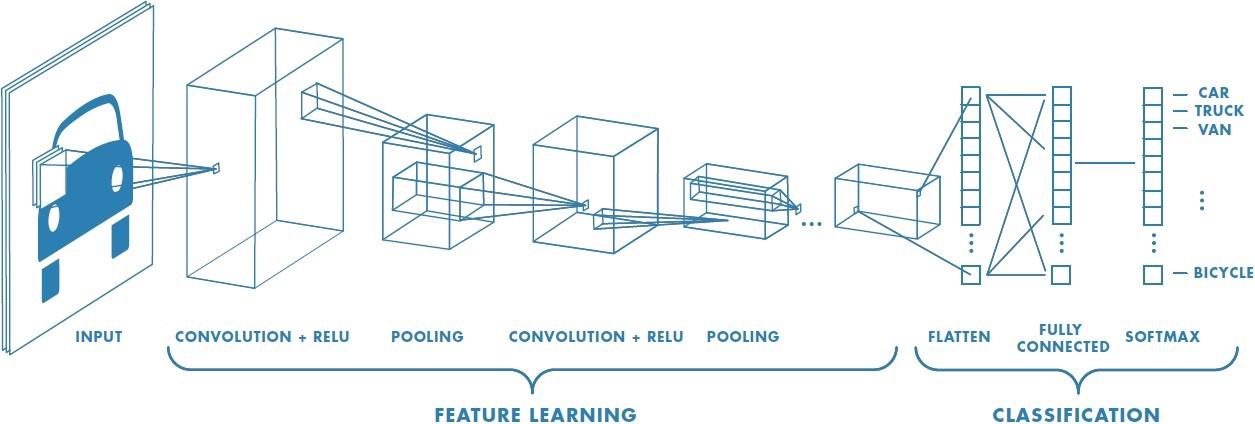
\includegraphics[width=17cm]{slike/CNNFull.jpeg}
\caption{Arhitektura konvolucijske neuronske mreže \citep{towardsDSCNN}}
\label{fig:fer-logo}
\end{figure}
\textbf{}


\section{Primjena u računalnom vidu i semantičkoj segmentaciji}
U ovom poglavlju ćemo pogledati kako se duboke neuronske mreže mogu iskoristiti za semantičku segmentaciju. Naglasak će biti na arhitekturama modificiranih konvolucijskih neuronskih mreža.

Generalni pristup semantičkoj segmentaciji korištenjem dubokih konvolucijskih modela možemo razdvojiti u dvije bitne komponente - \textbf{enkoder}, iza kojeg slijedi \textbf{dekoder}. Zadaća enkodera je obaviti klasifikaciju ulazne slike, na način opisan u poglavlju 3.2, no umjesto da rezultat klasifikacije koristeći potpuno povezani sloj dovedemo na izlaz mreže kao odluku o klasifikaciji slike, dovodimo ga na ulaz dekodera. Zatim je zadaća dekodera da naučenu klasifikaciju niže rezolucije projektira na izlaznu matricu, odnosno sliku, kako bi dobili gušću klasifikaciju, te u konačnici segmentacijsku mapu. Naravno, ovo je vrlo poopćen opis, te konkretni implementacijski detalji ovise o korištenoj arhitekturi.

U nastavku ćemo pogledati par istaknutih dubokih konvolucijskih modela koji, među ostalim, imaju primjenu u računalnom vidu i semantičkoj segmentaciji


\subsection{ResNet}
ResNet je, uz AlexNet, jedan od najpoznatijih dubokih modela u svijetu računalnog vida. Ova mreža je poznata po svojoj velikoj dubini (152 sloja), te uvođenju koncepta rezidualne jedinice.

ResNet kreće od ideje da, iako povećanje dubine mreže rezultira boljim performansama, također otežava treniranje. Ovo je najviše zbog pojave problema nestajućeg gradijenta (već spomenut u poglavlju 3.2.1), te slične pojave zvane eksplodirajući gradijent \engl{exploding gradient}. Oba ova problema postaju izraženija povećanjem dubine mreže.

Kako bi riješili ovaj problem, originalni autori uvode pojam \textbf{rezidualne jedinice} \engl{residual block}, prikazanog na slici 3.7 Na slici vidimo da se ulazni podaci, prilikom ulaska u neki od konvolucijskih slojeva, također nepromijenjeni šalju nekoliko slojeva dalje. Ovo je korisno zato što omogućava lakšu propagaciju gradijenta prilikom propagacije pogreške unazad. Konkretan primjer - ako jedan od konvolucijskih slojeva radi više štete nego koristi - recimo vodi do povećavanja funkcije pogreške umjesto smanjenja, koristeći ResNet arhitekturu praktički ga možemo ignorirati, jer imamo drugi put do ostatka mreže, stvoren grananjem rezidualne jedinice. Također, pošto je taj "alternativni" put ustvari put prema nepromijenjenom ulazu, ako odaberemo taj put efektivno smanjujemo dubinu mreže. Na ovaj način, dodatni slojevi mreže se koristi samo ukoliko pomaže u smanjenju funkcije gubitka. Ukoliko ne pomažu, mreža modificira težine na takav način da se prilikom dolaska do te rezidualne jedince uvijek odabere "zaobilazni" put, te na taj način efektivno smanji dubina mreže. U originalnom radu, \citep{resnetOriginal} ResNet arhitektura je korištena za problem klasifikacije slika, no manjim modifikacijama arhitekture te uvođenjem dekodera, primjenjiva je i za probleme semantičke segmentacije.

ResNet nije glavna tema ovog rada, stoga u dodatne implementacijske detalje neću ulaziti, no zainteresiranom čitatelju za daljnje istraživanje preporučujem originalni članak o ResNet arhitekturi \citep{resnetOriginal}, te članak \citep{resnetDecodingArhitecture}, koji na razumljiv i čitak način objašnjavaju ključne komponente arhitekture.

\begin{figure}[htb]
\centering
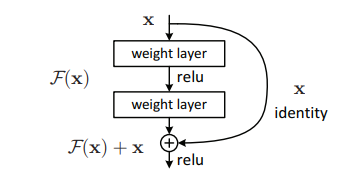
\includegraphics[width=13cm]{slike/resnet.png}
\caption{Rezidualna jedinica, ključna komponenta ResNet arhitekture \citep{resnetOriginal}}
\label{fig:fer-logo}
\end{figure}
\textbf{}\\


\subsection{U-net}
Osnovna motivacija nastanka U-net arhitekture je bila omogućiti dobre rezultate semantičke segmentacije uz relativno malenu količinu podataka. Razvijena je s ciljem segmentacije medicinskih slika, te je u tom području pokazala vrlo dobre rezultate. Formalno, ova arhitektura pripada u tzv. \textbf{potpuno konvolucijske mreže} \engl{fully convoluted neural networks, FCNN}, konvolucijske mreže koje se sastoje samo od konvolucijskih slojeva i slojeva sažimanja.

Najbolji način za razumijevanje arhitekture ove mreže je kroz skicu arhitekture, prikazanu na slici 3.8

\begin{figure}[htb]
\centering
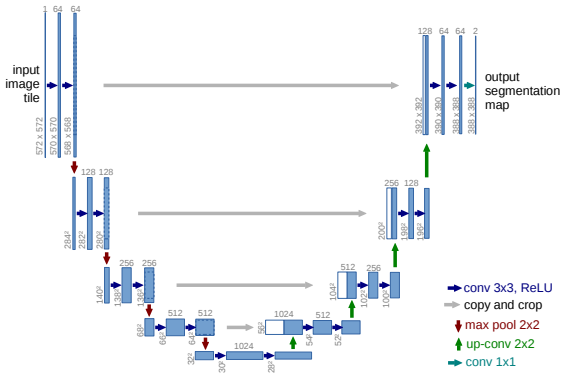
\includegraphics[width=13cm]{slike/unet.png}
\caption{U-net arhitektura. \citep{unetOriginal}}
\label{fig:fer-logo}
\end{figure}
\textbf{}

\noindent Na slici, svaki plavi kvadrat predstavlja višekanalnu mapu atributa. Broj na vrhu kvadrata predstavlja broj kanala u mapi, dok je sa strane dana i dimenzija mape. Strelicama različitih boja označene su operacije unutar mreže (legenda na slici).

Vidimo da se mreža sastoji od dva suprotna dijela - enkoderski dio, u kojem ulazna slika prolaskom kroz konvolucijske slojeve i slojeve sažimanja biva sve više i više poduzorkovana \engl{downsampling}. Ovime dobivamo mapu značajki malih dimenzija pomoću koje model može raspoznati veća grupiranja piksela iste klase na ulaznoj slici. Međutim, kako je dobivena slika vrlo malih dimenzija, potrebno je provesti proces naduzorkovanja \engl{upsampling}, u kojem se, koristeći proces "obrnute konvolucije", slici povećava rezolucija. Kako ne bi došlo do prekomjernog gubitka informacija prilikom povećanja rezolucije, koristan je velik broj kanala koji svaka mapa atributa ima. U zadnjem sloju dekoderskog dijela završavamo s mapom atributa jednake rezolucije kao i ulazna slika. U tom sloju se dodatno provodi 1x1 konvolucija, koja kao cilj ima mapirati dobivenu mapu atributa u odgovarajući broj klasa.

Prilikom treniranja, autori predlažu korištenje procesa augmentacije podataka, kako bi se poboljšalo svojstvo generalizacije mreže i smanjila količina potrebnih podataka.


\subsection{Deeplab}
Deeplab je zajednički naziv za obitelj dubokih neuronskih mreža razvijanih od strane Googlea. Trenutno postoje 4 verzije Deeplab arhitekture, od kojih je najnoviji DeeplabV3+ iz 2018.

U svojoj osnovi, Deeplab je modifikacija ResNet arhitekture, gdje se za proces enkodiranja, odnosno poduzorkovanja koristi manji broj slojeva sažimanja u kombinaciji sa \textbf{ dilatiranom konvolucijom} \engl{atrous convolution}. Ova vrsta konvolucija omogućava obrade većeg dijela slike manjom jezgrom, odnosno polje slike nad kojim se primjenjuje konvolucija ima veće dimenzije od same jezgre. Nedostajući podaci se nadopunjuju nulama. Parametar koji određuje stupanj dilatacije konvolucije naziva se \textbf{stopa dilatacije}. Primjerice, jezgra dimenzija 3x3 sa stopom dilatacije 2 pokriva područje veličine 5x5 originalne slike. Ovakav pristup omogućava pokrivanje većeg dijela slike koristeći konvoluciju s manjim brojem parametara. U Deeplab arhitekturi ovo svojstvo iskorištavamo tako da originalnu sliku poduzorkujemo manji broj puta nego što je to slučaj u ostalim arhitekturama. Umjesto toga, "povećavamo" efektivnu veličinu filtera koristeći dilatirane konvolucije umjesto običnih, te zatim te filtere primjenjujemo nad poduzorkovanim slikama. Primijetimo, dvije su glavne prednosti ovog pristupa: \citep{towardsDeeplab}

\begin{enumerate}
  \item Smanjenjenjem potrebnog broja operacija poduzorkovanja, ubrzavamo rad modela
  \item Kako konvolucije sad provodimo na slikama većih dimenzija (zbog manjeg broja poduzorkovanja), ovo nam omogućava da primjenom filtera izvučemo više značajki iz njih nego što je slučaj sa slikama manjih dimenzija, te samim time dobijemo točniju mapu značajki
\end{enumerate}
 
 DeeplabV2 i DeeplabV3 uvode još nekoliko modifikacija, poput piramidalnog dilatiranog sažimanja i oštrije detekcije rubova na slikama.
